% Copyright (c)  2019  FSC.
% Permission is granted to copy, distribute and/or modify this document
% under the terms of the GNU Free Documentation License, Version 1.3
% or any later version published by the Free Software Foundation;
% with no Invariant Sections, no Front-Cover Texts, and no Back-Cover Texts.
% A copy of the license is included in the section entitled "GNU
% Free Documentation License".

\chapter{Sviluppo del sito}\label{chap:sviluppo-sito}
In questa fase, vengono descritte in dettaglio le funzioni precisando gli 
scenari di esecuzione di tutti i casi d'uso introdotti nalla fase dei 
requisiti. Si sono costruiti dei diagrammi di navigazione attraverso i 
diagrammi per macchine a stati. 

% Copyright (c)  2019  FSC.
% Permission is granted to copy, distribute and/or modify this document
% under the terms of the GNU Free Documentation License, Version 1.3
% or any later version published by the Free Software Foundation;
% with no Invariant Sections, no Front-Cover Texts, and no Back-Cover Texts.
% A copy of the license is included in the section entitled "GNU
% Free Documentation License".

\begin{figure}[H]
	\centering
	\caption{Diagramma macchine a stati del caso d'uso 'Registration'.}
	\label{fig:diagramma-macchine-stati:registration}
	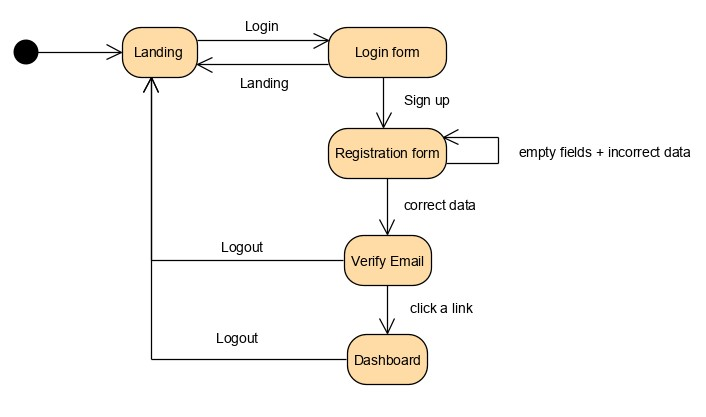
\includegraphics[width=\textwidth]{images/diagramma-macchine-stati/registration}
\end{figure}

\begin{figure}[H]
	\centering
	\caption{Diagramma macchine a stati del caso d'uso 'Login'.}
	\label{fig:diagramma-macchine-stati:login}
	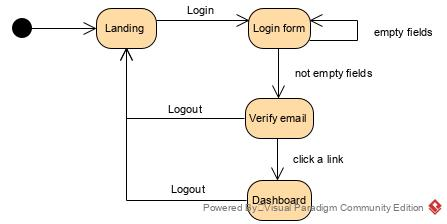
\includegraphics[width=\textwidth]{images/diagramma-macchine-stati/login}
\end{figure}
\begin{figure}[H]
	\centering

	\caption{Diagramma macchine a stati del caso d'uso 'Logout'.}
	\label{fig:diagramma-macchine-stati:logout}
	
\includegraphics[width=\textwidth]{images/diagramma-macchine-stati/logout}
\end{figure}

\begin{figure}[H]
	\centering
	\caption{Diagramma macchine a stati del caso d'uso 'Create project'.}
	\label{fig:diagramma-macchine-stati:create-project}
	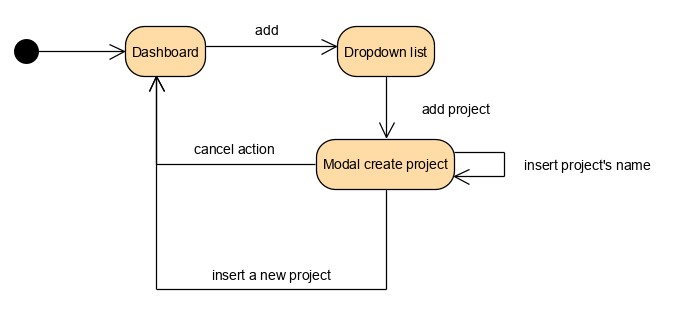
\includegraphics[width=\textwidth]{images/diagramma-macchine-stati/create-project}
\end{figure}

\begin{figure}[H]
	\centering
	\caption{Diagramma macchine a stati del caso d'uso 'View project'.}
	\label{fig:diagramma-macchine-stati:view-project}
	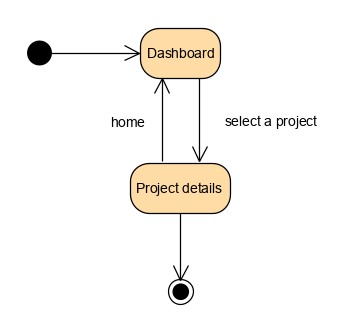
\includegraphics[width=\textwidth]{images/diagramma-macchine-stati/view-project}
\end{figure}

\begin{figure}[H]
	\centering
	\caption{Diagramma macchine a stati del caso d'uso un video.}
	\label{fig:diagramma-macchine-stati:video}
	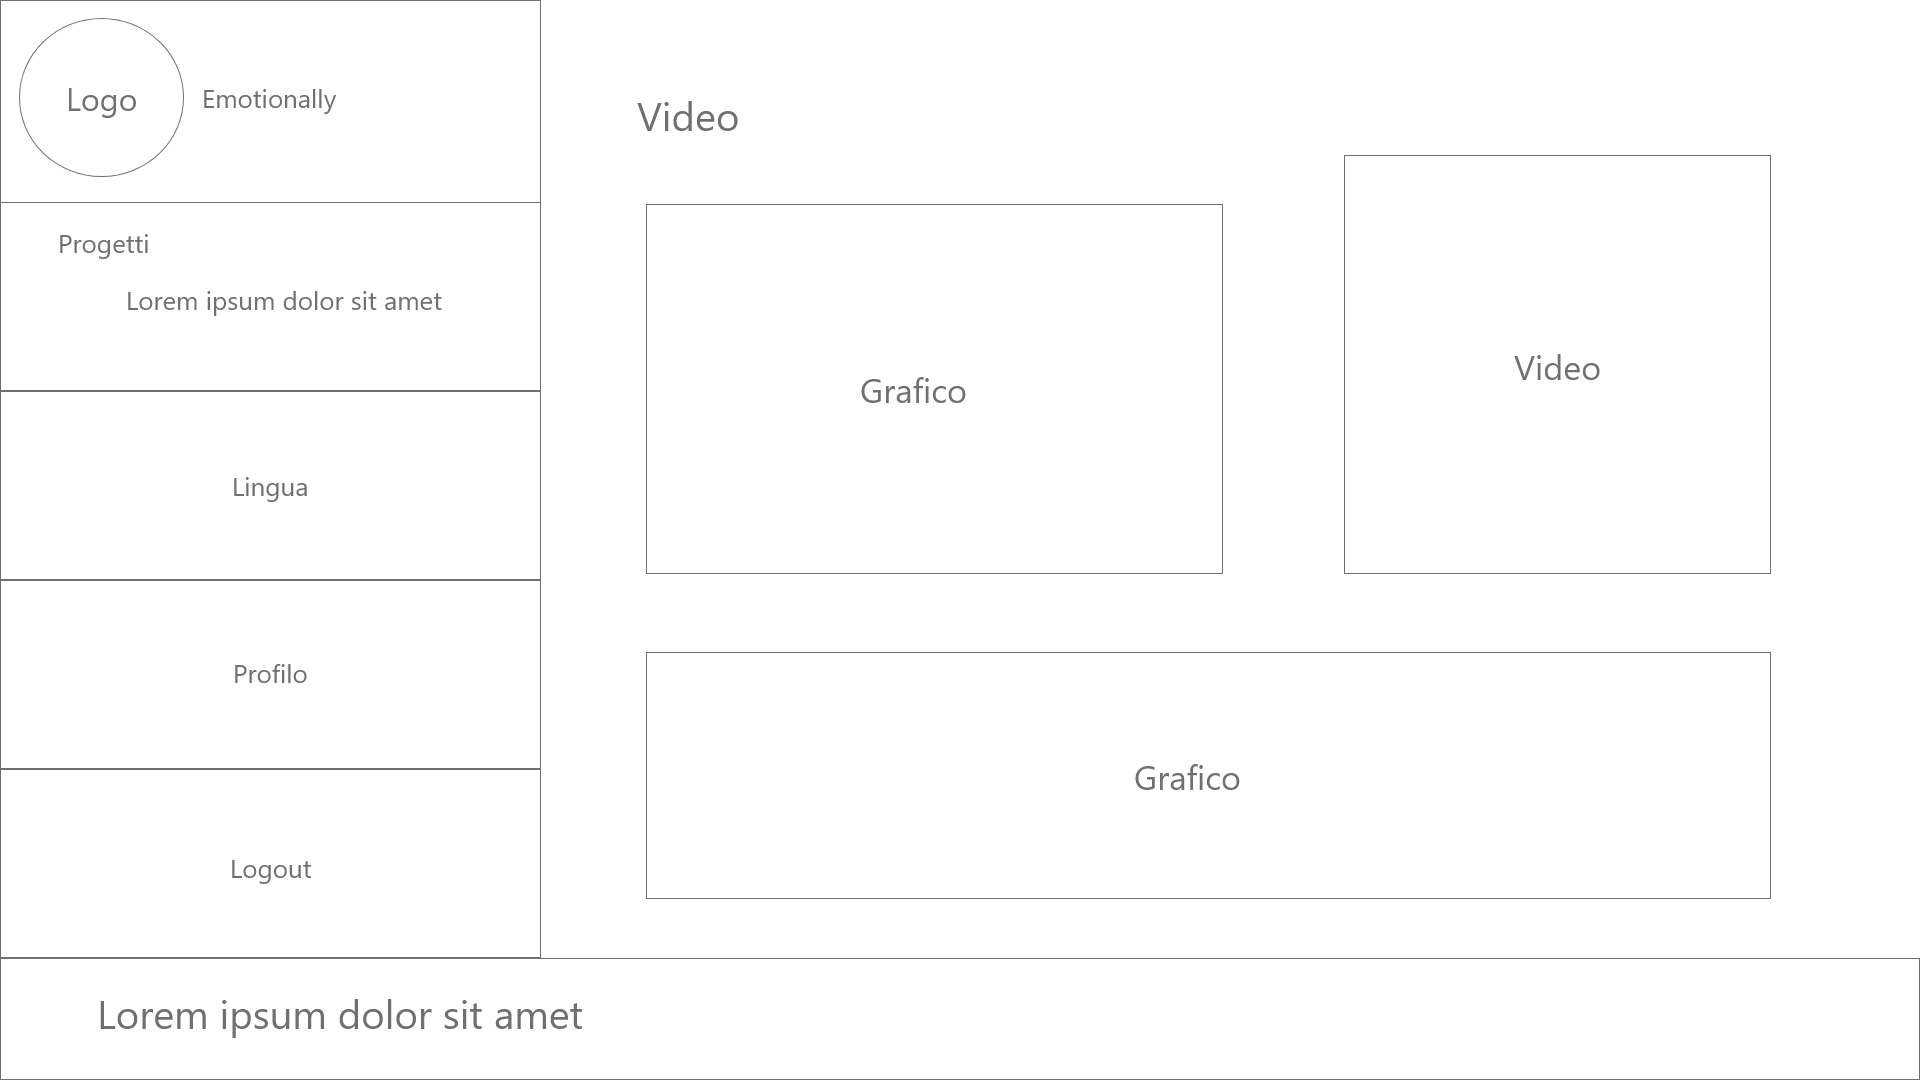
\includegraphics[width=\textwidth]{images/diagramma-macchine-stati/Video}
\end{figure}

\begin{figure}[H]
	\centering
	\caption{Diagramma macchine a stati del caso d'uso 'Edit project'.}
	\label{fig:diagramma-macchine-stati:edit-project}
	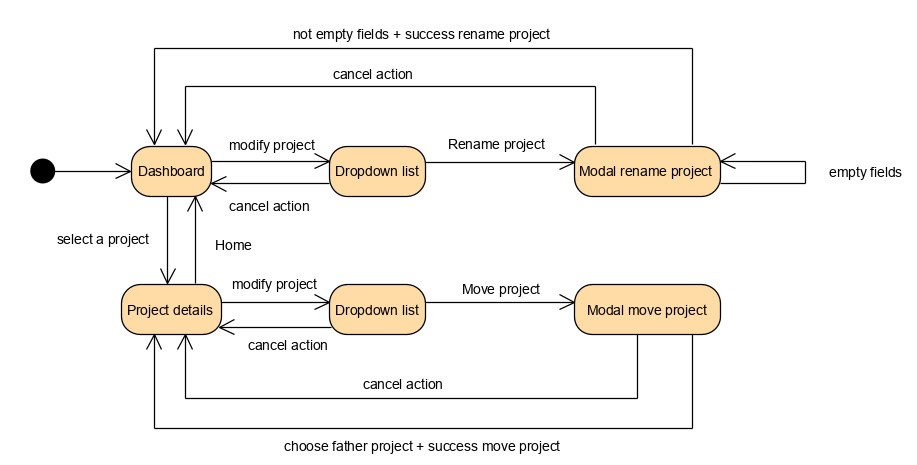
\includegraphics[width=\textwidth]{images/diagramma-macchine-stati/edit-project}
\end{figure}

\begin{figure}[H]
	\centering
	\caption{Diagramma macchine a stati del caso d'uso 'Remove project'.}
	\label{fig:diagramma-macchine-stati:remove-project}
	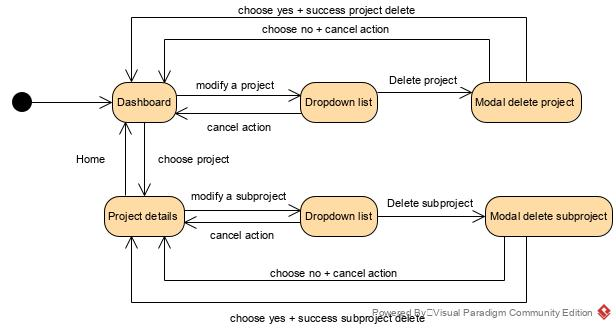
\includegraphics[width=\textwidth]{images/diagramma-macchine-stati/remove-project}
\end{figure}

\begin{figure}[H]
	\centering
	\caption{Diagramma macchine a stati del caso d'uso 'Upload video'.}
	\label{fig:diagramma-macchine-stati:upload-video}
	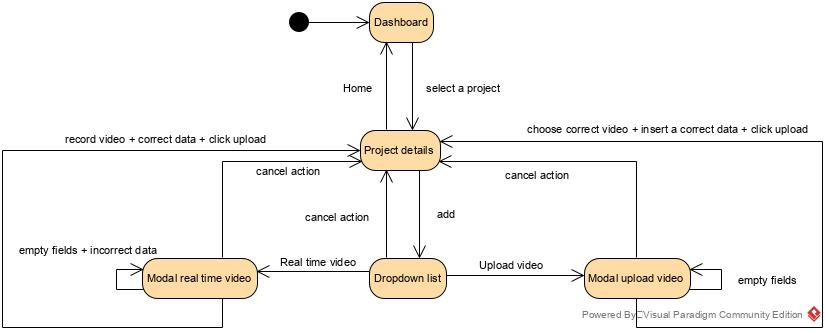
\includegraphics[width=\textwidth]{images/diagramma-macchine-stati/upload-video}
\end{figure}

\begin{figure}[H]
	\centering
	\caption{Diagramma macchine a stati del caso d'uso 'Edit video'.}
	\label{fig:diagramma-macchine-stati:edit-video}
	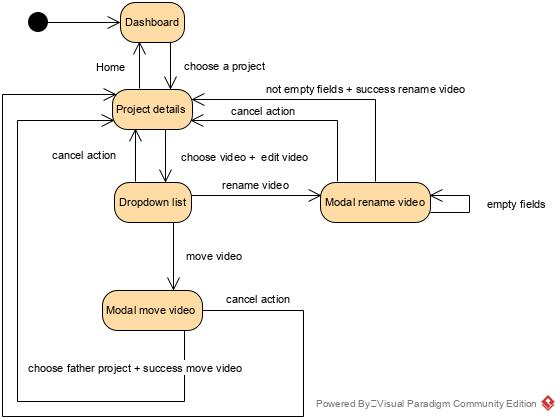
\includegraphics[width=\textwidth]{images/diagramma-macchine-stati/edit-video}
\end{figure}

\begin{figure}[H]
	\centering
	\caption{Diagramma macchine a stati del caso d'uso 'Remove video'.}
	\label{fig:diagramma-macchine-stati:remove-video}
	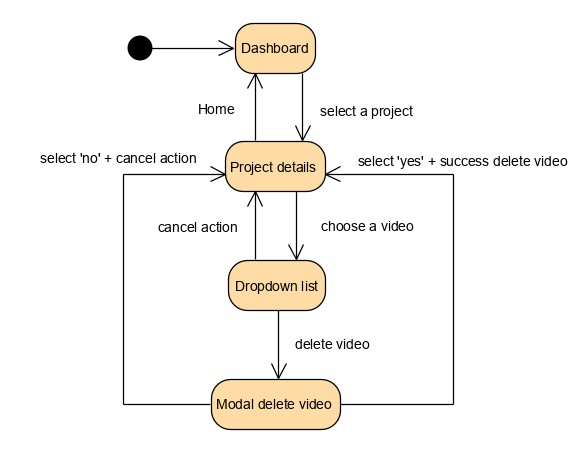
\includegraphics[width=\textwidth]{images/diagramma-macchine-stati/remove-video}
\end{figure}

\begin{figure}[H]
	\centering
	\caption{Diagramma macchine a stati del caso d'uso 'View video'.}
	\label{fig:diagramma-macchine-stati:view-video}
	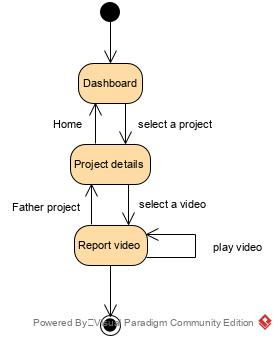
\includegraphics[width=\textwidth]{images/diagramma-macchine-stati/view-video}
\end{figure}

\begin{figure}[H]
	\centering
	\caption{Diagramma macchine a stati del caso d'uso 'Share project'.}
	\label{fig:diagramma-macchine-stati:share-project}
	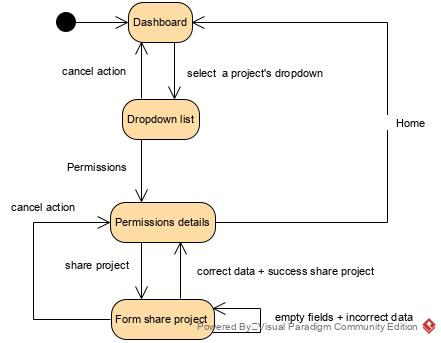
\includegraphics[width=\textwidth]{images/diagramma-macchine-stati/share-project}
\end{figure}

\begin{figure}[H]
	\centering
	\caption{Diagramma macchine a stati del caso d'uso 'Update user data'.}
	\label{fig:diagramma-macchine-stati:update-user-data}
	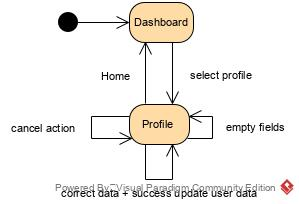
\includegraphics[width=\textwidth]{images/diagramma-macchine-stati/update-user-data}
\end{figure}

\begin{figure}[H]
	\centering
	\caption{Diagramma macchine a stati del caso d'uso 'View report of a 
	video'.}
	\label{fig:diagramma-macchine-stati:view-report-video}
	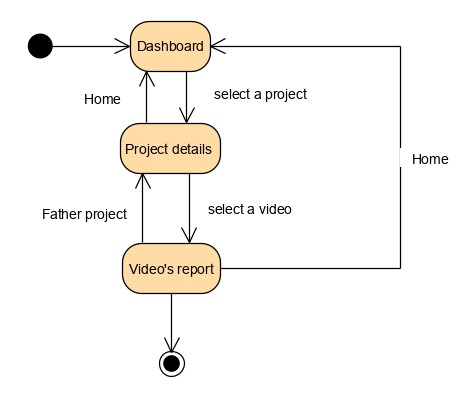
\includegraphics[width=\textwidth]{images/diagramma-macchine-stati/view-report-video}
\end{figure}

\begin{figure}[H]
	\centering
	\caption{Diagramma macchine a stati del caso d'uso 'View report of a 
	project'.}
	\label{fig:diagramma-macchine-stati:view-report-project}
	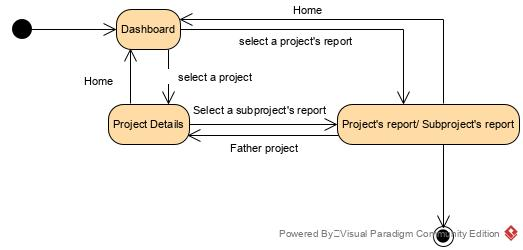
\includegraphics[width=\textwidth]{images/diagramma-macchine-stati/view-report-project}
\end{figure}

\begin{figure}[H]
	\centering
	\caption{Diagramma macchine a stati del caso d'uso 'Download report'.}
	\label{fig:diagramma-macchine-stati:download-report}
	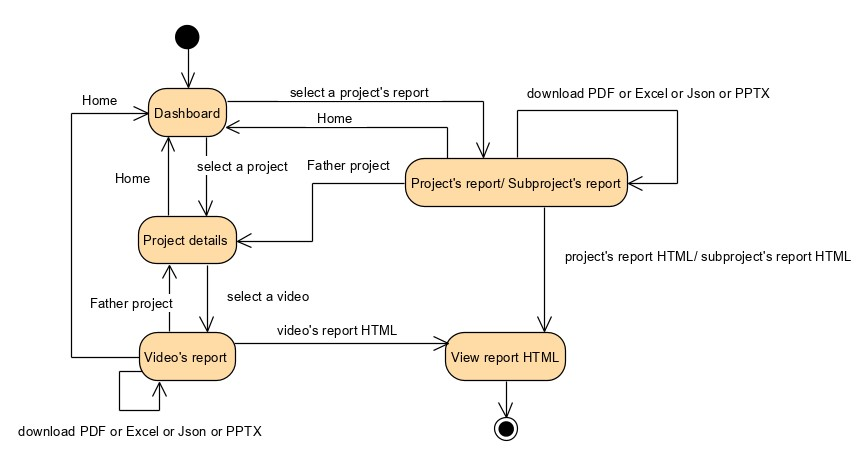
\includegraphics[width=\textwidth]{images/diagramma-macchine-stati/download-report}
\end{figure}

\section{Struttura dei form}\label{sec:struttura-form}

% Copyright (c)  2019  FSC.
% Permission is granted to copy, distribute and/or modify this document
% under the terms of the GNU Free Documentation License, Version 1.3
% or any later version published by the Free Software Foundation;
% with no Invariant Sections, no Front-Cover Texts, and no Back-Cover Texts.
% A copy of the license is included in the section entitled "GNU
% Free Documentation License".

\begin{figure}[H]
	\centering
	\caption{Struttura del form relativo all'aggiunta di un nuovo progetto.}
	\label{fig:struttura-form:aggiunta-progetto}
	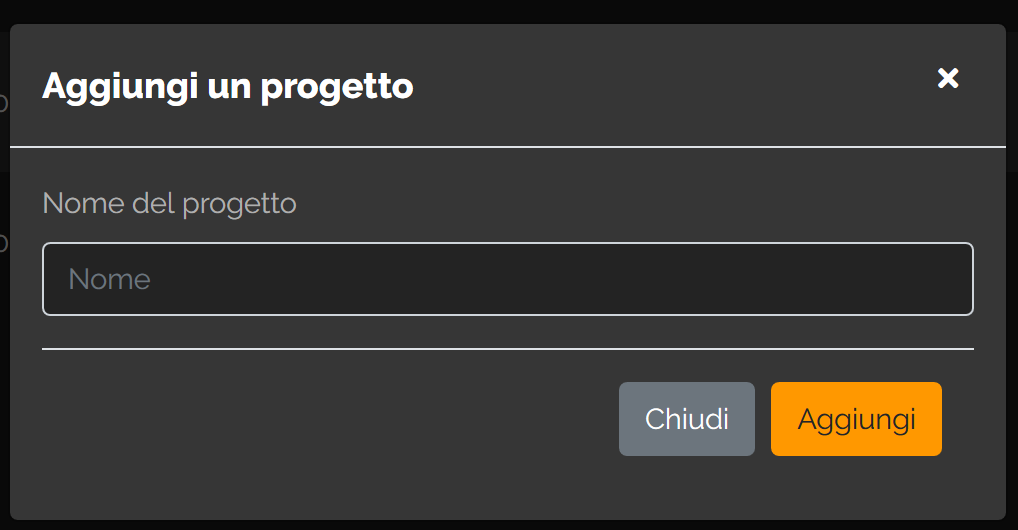
\includegraphics[width=\textwidth]{images/struttura-form/form-aggiungi-progetto}
\end{figure}

\begin{figure}[H]
	\centering
	\caption{Struttura del form relativo al rimonima progetto.}
	\label{fig:struttura-form:rinomina-progetto}
	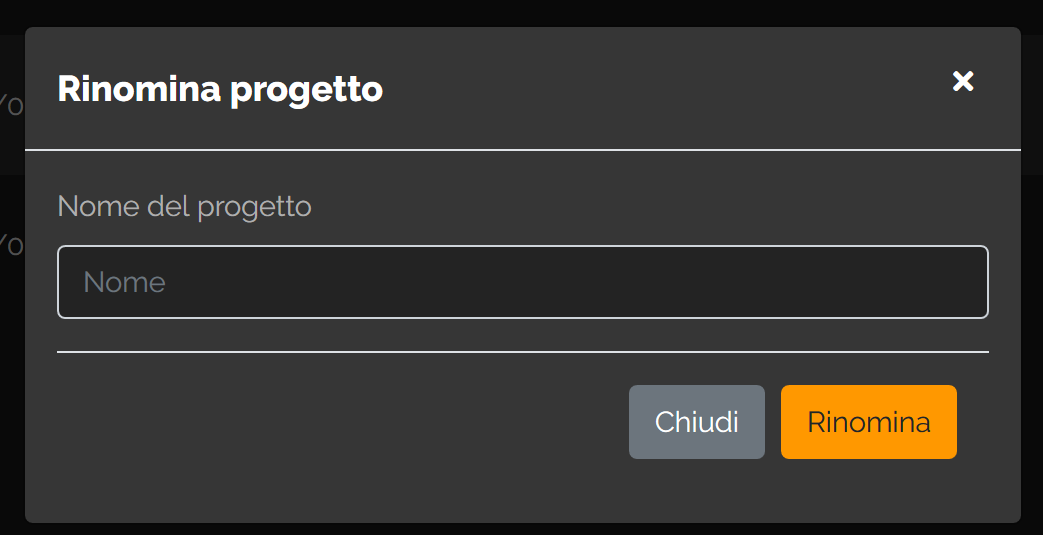
\includegraphics[width=\textwidth]{images/struttura-form/form-rinomina-progetto}
\end{figure}

\begin{figure}[H]
	\centering

	\caption{Struttura del form relativo al caricamento di un video.}
	\label{fig:struttura-form:carica-video}
	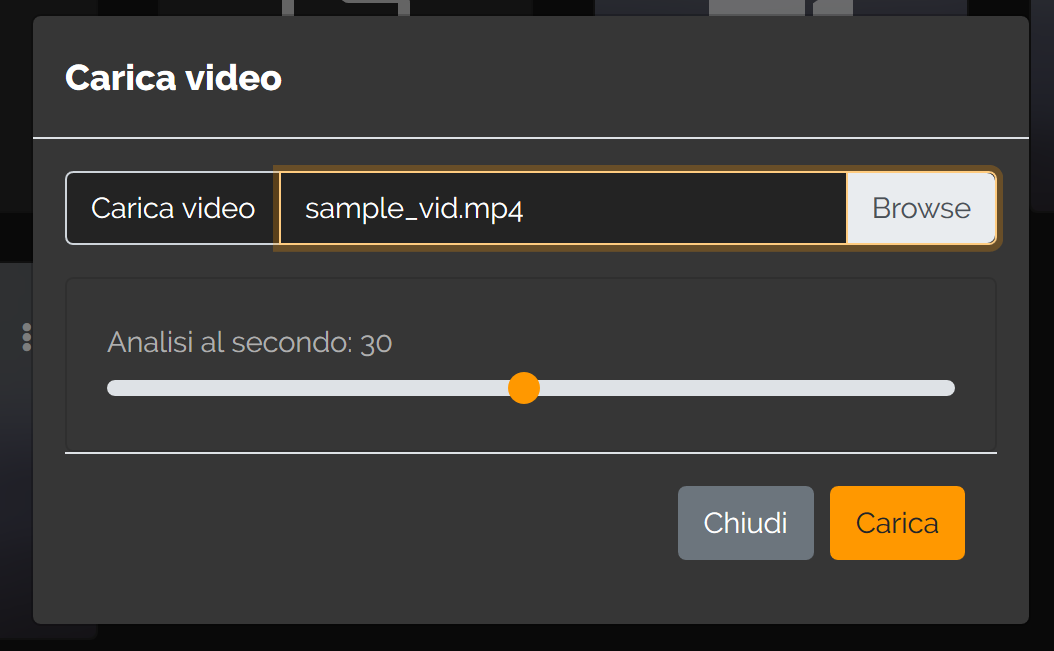
\includegraphics[width=\textwidth]{images/struttura-form/form-carica-video}
\end{figure}

\begin{figure}[H]
	\centering
	\caption{Struttura del form relativo al caricamento di un video real time.}
	\label{fig:struttura-form:carica-video-realtime}
	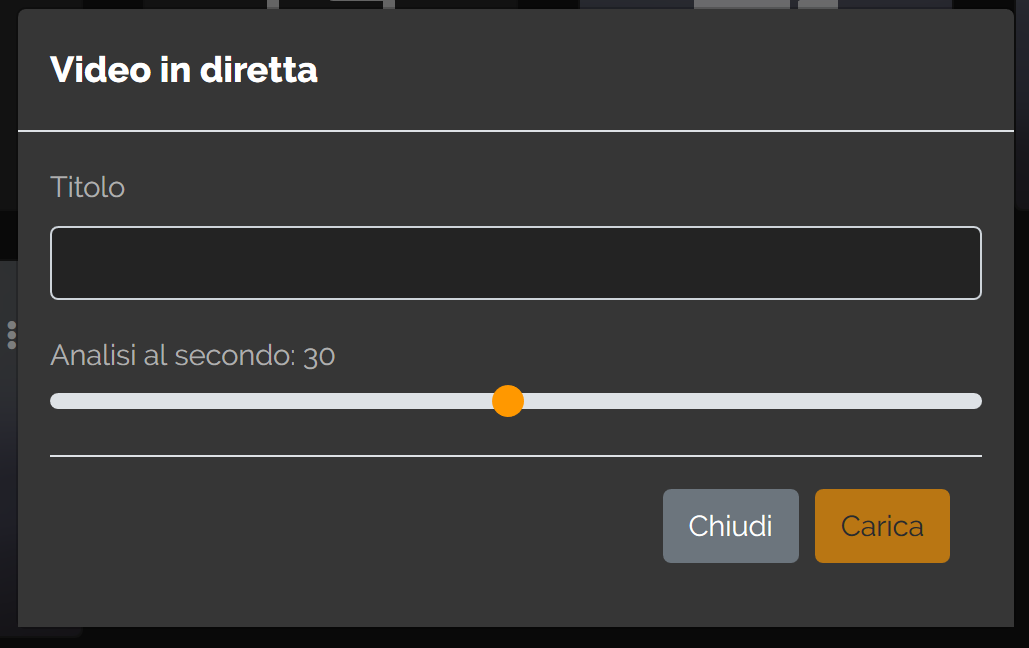
\includegraphics[width=\textwidth]{images/struttura-form/form-video-diretta}
\end{figure}

\begin{figure}[H]
	\centering
	\caption{Struttura del form relativo al login.}
	\label{fig:struttura-form:login}
	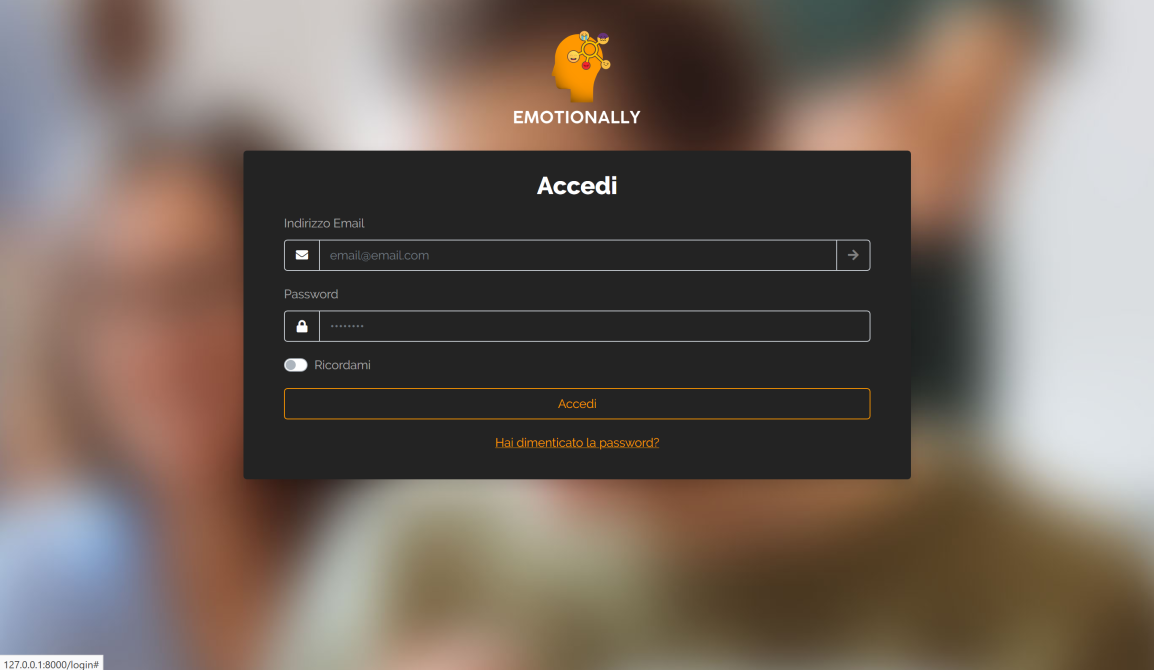
\includegraphics[width=\textwidth]{images/struttura-form/form-login}
\end{figure}

\begin{figure}[H]
	\centering
	\caption{Struttura del form relativo alla modifica dei dati di un account.}
	\label{fig:struttura-form:modifica-dati-account}
	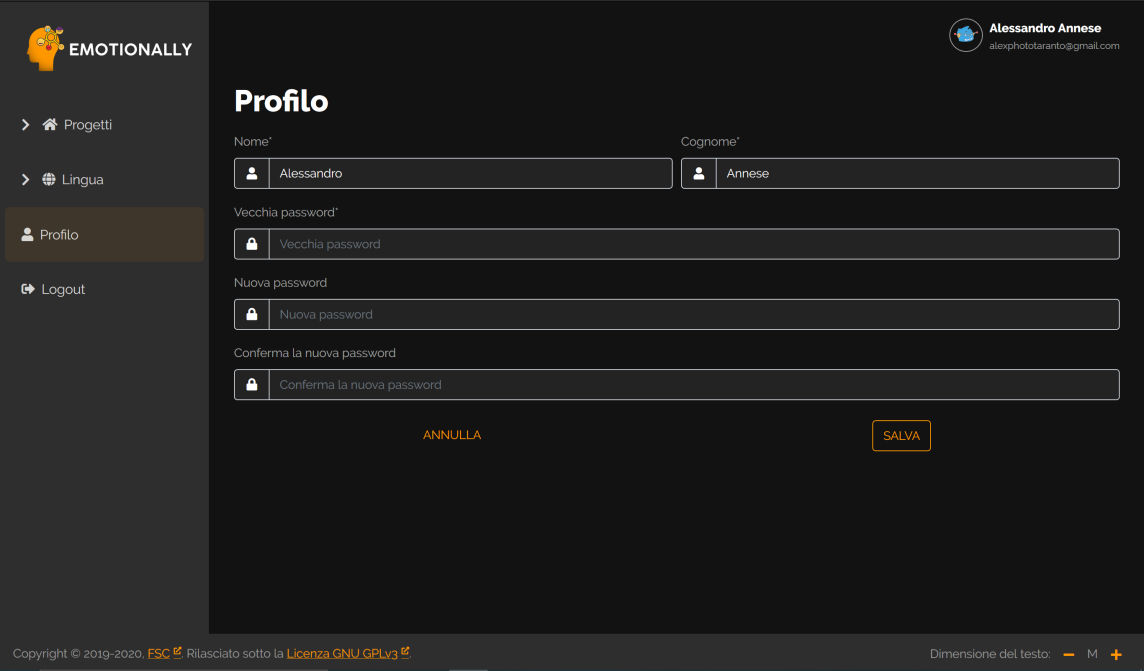
\includegraphics[width=\textwidth]{images/struttura-form/form-modifica-account}
\end{figure}

\begin{figure}[H]
	\centering
	\caption{Struttura del form relativo alla registrazione.}
	\label{fig:struttura-form:registrazione}
	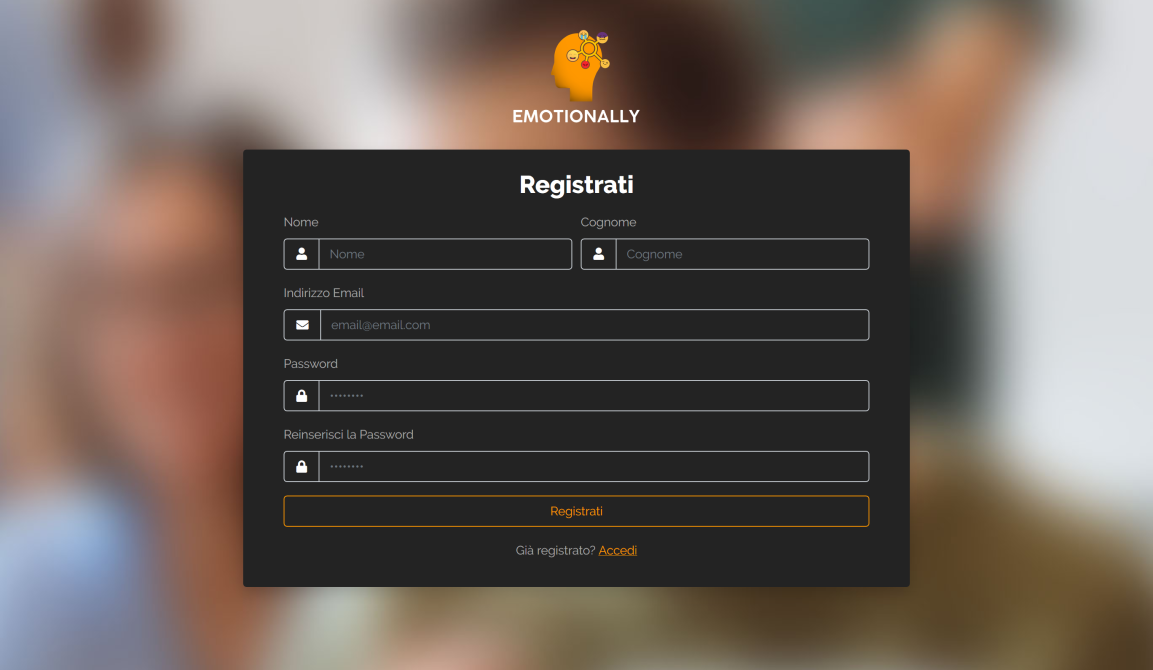
\includegraphics[width=\textwidth]{images/struttura-form/form-registrazione}
\end{figure}

\begin{figure}[H]
	\centering
	\caption{Struttura del form relativo al reimposta password.}
	\label{fig:struttura-form:reimposta-password}
	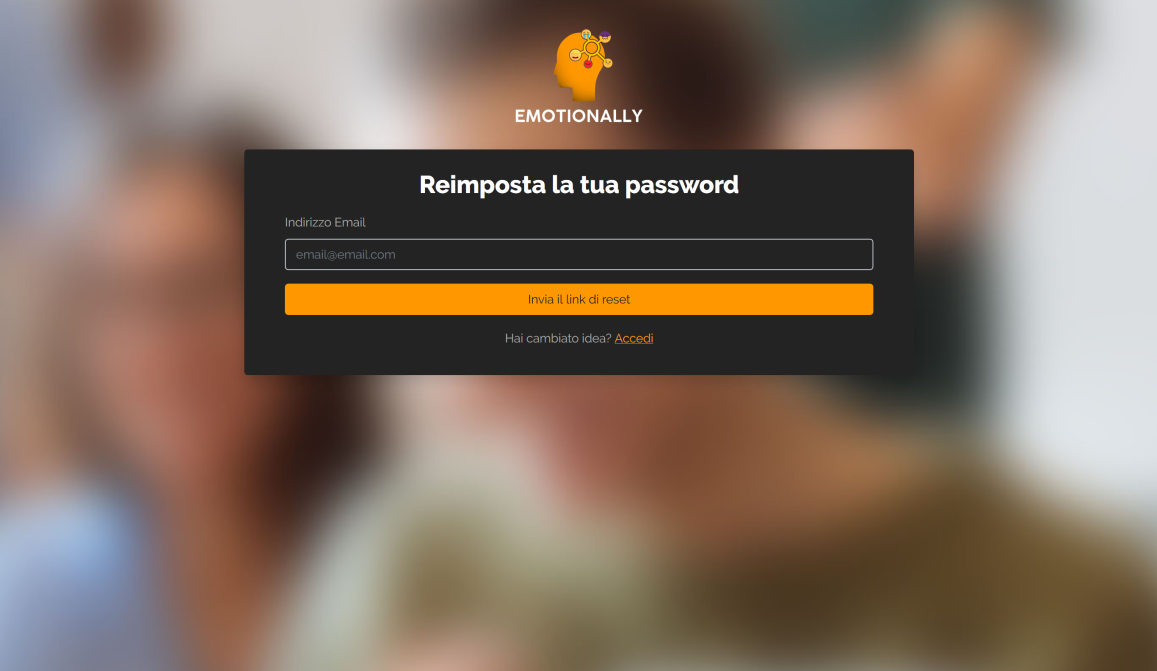
\includegraphics[width=\textwidth]{images/struttura-form/form-reimposta-password}
\end{figure}

\begin{figure}[H]
	\centering
	\caption{Struttura del form relativo al reset password.}
	\label{fig:struttura-form:reset-password}
	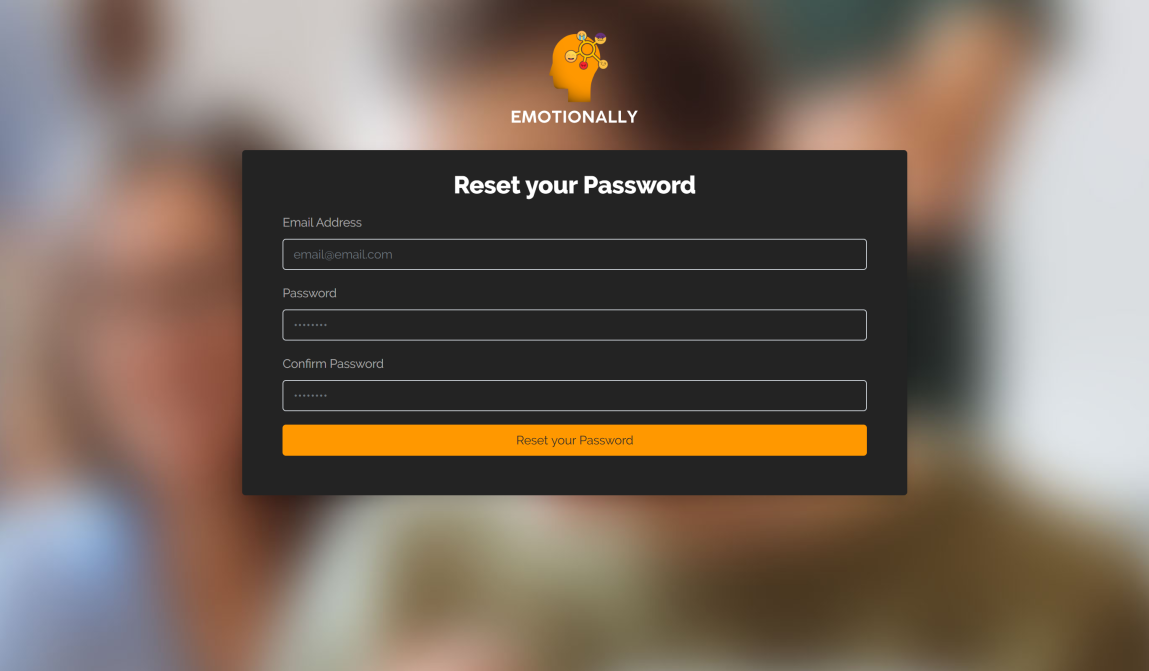
\includegraphics[width=\textwidth]{images/struttura-form/form-reset-password}
\end{figure}



\section{Modello logico base di dati}\label{sec:modello-logico}

\begin{figure}[H]
	\centering
	\caption{Modello logico della base di dati del sistema.}
	\label{fig:logical-diagram}
	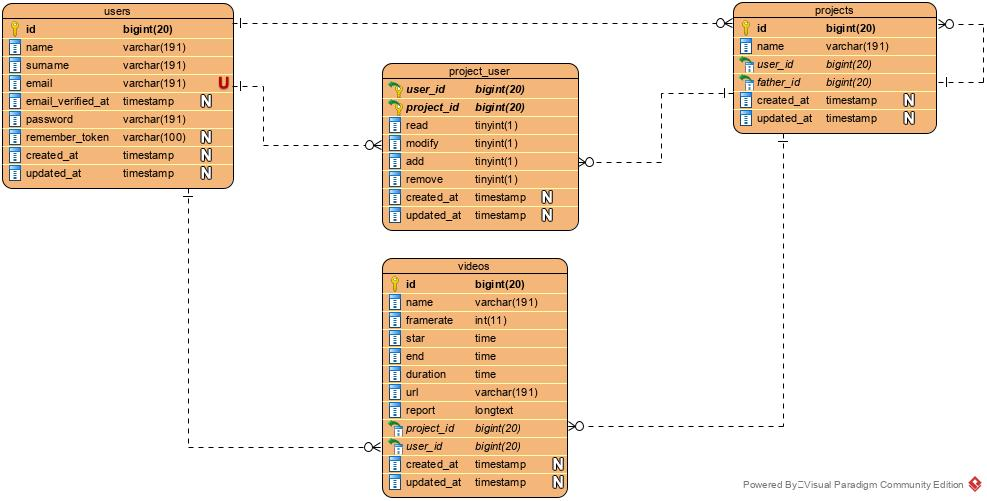
\includegraphics[width=\textwidth]{images/logical-diagram}
\end{figure}

